\documentclass{report}
\usepackage[utf8]{inputenc}
\usepackage{amsmath}
\usepackage{graphicx}

\title{Eksamensnoter - Divide and Conquer}
\author{André Oskar Andersen (wpr684)}
\date{\today}

\begin{document}
\maketitle

\section*{15 Dynamic Pgoramming}
\begin{itemize}
    \item Dynamic programming, like the divide-and-conquer method, solves problems by dombining the solutions to subproblems. Dynamic programming applies when the subproblems overlap - that is, when subproblems share subsubproblems. A dynamic-programming algorithm solves each subsubproblem just once and then saves its answer in a table, thereby avoiding the work of recomputing the answer every time it solves each subsubproblem
\end{itemize}

\subsection*{15.1 Rod cutting}
\begin{itemize}
    \item Our first example uses dynamic programming to solve a simple problem in deciding where to cut steel rods. Serling Enterprises buys long steel rods and cuts them into shorter rods, which it then sells. Each cut is free. The management of Serling Enterprises wants to know the best way to cut up the rods
    \item We assume that we know for $i = 1, 2, ...$ the price $p_i$ in dollars that Serling Enterprises charges for a rod of length \textit{i} inches.
    \item The \textit{rod-cutting problem} is as following. Given a rod of length \textit{n} inches and a table of prices $p_i$ for $i = 1, 2, ..., n$, determine the maximum revenue $_n$ obtainable by cutting up the rod and selling the pieces. We can cut up a rod of length \textit{n} in $2^{n - 1}$ different ways, since we have an independent option of cutting, or not cutting, at distance \textit{i} inches from the left end, for $i = 1, 2, ..., n - 1$. If an optimal solution cuts the rod into \textit{k} pieces, for some $1 \leq k \leq n$, then an optimal decomposition $n = i_1 + i_2 + ... + i_k$ of the rod into pieces of length $i_1, i_2, ..., i_k$ provides maximum corresponding revenue $r_n = p_{i_1} + p_{i_2} + p_{i_k}$. 
    More generally, we can frame the values $r_n$ for $n \geq 1$ in terms of optimal revenues fro mshorter rods: 
    $$r_n = \max(p_n, r_1 + r_{n - 1}, r_2 + r_{n - 2}, ..., r_{n - 1} + r_1)$$
    The first argument, $p_n$, corresponds to making no cuts at all and selling the rod of length \textit{n} as is. The other $n - 1$ arguments to max correspond to the maximum revenue obtained by making an initial cut of the rod into two pieces of size \textit{i} and $n - i$, for each $i = 1, 2, ..., n - 1$, and then optimally cutting up those pieces further, obtaining revenues $r_i$ and $r_{n - 1}$ from those two pieces.
    We say that the rod-cutting problem exhibits \textit{optimal substructure}: optimal solutions to a problem incorporate optimal solutions to related subproblems, which we may solve independently.
    In a related way to arrange a recursive structure for the rod-cutting problem, we view a decomposition as consisting of a first piece of length \textit{i} cut off the left-hand end, and then a right-hand remainder of length $n - i$. Only the remainder, and not the first piece, may be further divided. We thus obtain the following simpler equation:
    $$r_n = \max_{1 \leq i \leq n} (p_i + r_{n - i})$$
    In this formulation, an optimal solution embodies the solution to only one related subproblem - the remainder - rather than two.
\end{itemize}
\textbf{Recursive top-down implementation}
\begin{itemize}
    \item There are $2^{n - 1}$ ways of cutting up \textit{R}, hence the this algorithm runs in exponential time
\end{itemize}
\textbf{Using dynamic programming for optimal rod cutting}
\begin{itemize}
    \item The dynamic-programming method works as follows. Having observed that anaive recursive solution is inefficient because it solves the same subproblems repeatedly, we arrange for each ubproblem to be solved only once, saving its solution. If we need to refer to this subproblem's solution again later, we can just look it up, rather than recompute it.
    \item There are usually two equivalent ways to implement a dynamic-programming approach:
    \begin{enumerate}
        \item The first approach is \textit{top-down with memoization}. In this approach, wewrite the procedure reursively in a natural manner, but modified to save the result of each subproblem. The procedure now first checks to see whether it has previously solved this subproblem. If so, it returns the saved value, saving further computation at this level; if not, the procedure computes the value in the usual manner. We say that the recursive procedure has been \textit{memoized}; it "remembers" what results it has computed previously
        \item The second approach is the \textit{bottom-up method}. This approach typically depends on some natural notion of the "size" of a subproblem, such that solving any particular subproblem depends only on solving "smaller" subproblems. We sort the subproblems by size and solve them in size order, smallest first. When solving a particular subproblem, we have already solved all of the smaller subproblems its solution depends upon, and we have saved their solutions. We solve each subproblem only once, and when we first see it, we have already solved all of its prerequisite subproblems.
    \end{enumerate}
    \item The two approaches have the same asymptotic running time; $\Theta(n^2)$
\end{itemize}
\textbf{Subproblem graph}
\begin{center}
    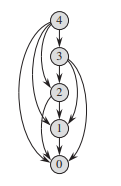
\includegraphics[height = 5 cm]{../entities/subproblem_graph.png}
\end{center}
\begin{itemize}
    \item The \textit{subproblem graph} for the problem embodies the set of subproblems involved and how subproblems depend on one another
\end{itemize}

\end{document}